The Higgs boson mass dependent signal selections in the cut-based analysis 
are described in Section~\ref{sec:anal_cutbased}. In this section we summarise 
the results obtained all jet final states. 
Tables~\ref{tab:yield_cutbased} shows the signal %equivalent data yields
and background expectations in ee and $\mu\mu$ final states.
The expected cross section ratio limits as a function of the Higgs mass, 
together with the 1/2-$\sigma$ uncertainty bands in Table~\ref{tab:limits_cutbased_4fb} and Figure~\ref{fig:limits_cut_4fb}. 


%%%%%%%%%%%%%%%%%%%%%%%%%
\begin{table}[!ht]
{\small
\begin{center}
 \begin{tabular}{l | c c |  c c c c c c | c }
 \hline\hline
 $m_H$ & qqH & ggH & qqZZ & ggZZ & WZ & WWTop & Zjets & $\sum$Bkg & Data \\
 \hline
\multicolumn{10}{c} {ee} \\ \hline
250 & $0.8\pm0.1$ & $7.7\pm1.2$ & $12.2\pm1.3$ & $1.1\pm0.3$ & $9.0\pm1.1$ & $24.1\pm0.0$ & $14.9\pm4.3$ & $61.4\pm4.6$ & 50 \\
300 & $0.8\pm0.1$ & $7.7\pm1.2$ & $8.3\pm0.9$ & $0.7\pm0.2$ & $5.3\pm0.7$ & $9.1\pm0.0$ & $5.3\pm1.4$ & $28.8\pm1.8$ & 24 \\
350 & $0.7\pm0.1$ & $7.9\pm1.3$ & $6.0\pm0.6$ & $0.5\pm0.1$ & $3.1\pm0.4$ & $1.4\pm0.0$ & $2.7\pm0.7$ & $13.7\pm1.1$ & 12 \\
400 & $0.5\pm0.1$ & $6.8\pm1.2$ & $4.6\pm0.5$ & $0.4\pm0.1$ & $2.2\pm0.3$ & $0.0\pm0.0$ & $1.9\pm0.6$ & $9.2\pm0.8$ & 9 \\
500 & $0.3\pm0.1$ & $3.1\pm0.7$ & $2.8\pm0.3$ & $0.2\pm0.0$ & $1.2\pm0.2$ & $0.0\pm0.0$ & $1.1\pm0.4$ & $5.4\pm0.5$ & 8 \\
600 & $0.2\pm0.1$ & $1.2\pm0.4$ & $1.5\pm0.2$ & $0.1\pm0.0$ & $0.6\pm0.1$ & $0.0\pm0.0$ & $0.9\pm0.3$ & $3.2\pm0.4$ & 1 \\
\hline
\multicolumn{10}{c} {$\mu\mu$} \\ 
\hline
250 & $1.1\pm0.1$ & $10.4\pm1.5$ & $17.4\pm1.7$ & $1.6\pm0.4$ & $12.7\pm1.5$ & $29.8\pm0.0$ & $23.4\pm6.7$ & $85.0\pm7.1$ & 78 \\
300 & $1.1\pm0.1$ & $10.2\pm1.5$ & $11.6\pm1.1$ & $1.0\pm0.2$ & $7.1\pm0.8$ & $11.1\pm0.0$ & $8.5\pm2.2$ & $39.2\pm2.7$ & 39 \\
350 & $0.9\pm0.1$ & $10.4\pm1.6$ & $7.9\pm0.8$ & $0.7\pm0.1$ & $4.3\pm0.5$ & $1.6\pm0.0$ & $4.2\pm1.1$ & $18.7\pm1.5$ & 17 \\
400 & $0.6\pm0.1$ & $9.0\pm1.5$ & $6.3\pm0.6$ & $0.5\pm0.1$ & $3.0\pm0.4$ & $0.0\pm0.0$ & $2.7\pm0.8$ & $12.5\pm1.1$ & 13 \\
500 & $0.4\pm0.1$ & $3.9\pm0.9$ & $4.0\pm0.4$ & $0.3\pm0.1$ & $1.5\pm0.2$ & $0.0\pm0.0$ & $1.6\pm0.5$ & $7.5\pm0.7$ & 8 \\
600 & $0.2\pm0.1$ & $1.5\pm0.5$ & $2.2\pm0.2$ & $0.2\pm0.0$ & $0.7\pm0.1$ & $0.0\pm0.0$ & $1.3\pm0.4$ & $4.3\pm0.5$ & 3 \\
\hline\hline
\end{tabular}
\end{center}
}
\caption{Expected number of signal and background events for an integrated luminosity of \intlumi after applying the higgs selections 
  in the cut-based analysis in the ee final state. Both statistical and systematic uncertainties are included. For the sum of the $\ww$ and Top backgrounds, the uncertainties are 
  not shown here which are modelled by a Gamma function of the number of $e\mu$ events in the control region.  }
\label{tab:yield_cutbased}
\end{table}

%%%%%%%%%%%%%%%%%%%%%%%%%%%%%%%
\begin{table}[!ht]
\begin{center}
\begin{tabular}{ccccc}
\hline\hline
Mass & Median Expected & [-$\sigma$, +$\sigma$] & [-2$\sigma$, +2$\sigma$]\\\hline
250 & 1.88 & [1.30, 2.75] & [0.94, 3.86] \\
300 & 1.15 & [0.81, 1.66] & [0.59, 2.31] \\
350 & 0.77 & [0.54, 1.10] & [0.40, 1.56] \\
400 & 0.77 & [0.54, 1.08] & [0.39, 1.50] \\
500 & 1.41 & [0.98, 2.01] & [0.73, 2.87] \\
600 & 3.12 & [2.18, 4.73] & [1.66, 6.89] \\
\hline\hline
\end{tabular}
\end{center}
\caption{The median expected cross section ratio limits as a function 
of the Higgs mass, together with the 1/2-$\sigma$ uncertainty bands obtained in the cut-and-count analysis, corresponding to 
an integrated luminosity of \intlumi}
\label{tab:limits_cutbased_4fb}
\end{table}

%%%%%%%%%%%%%%%%%%%%%%%%%%%%%
\begin{figure}[!htbp]
\begin{center}
   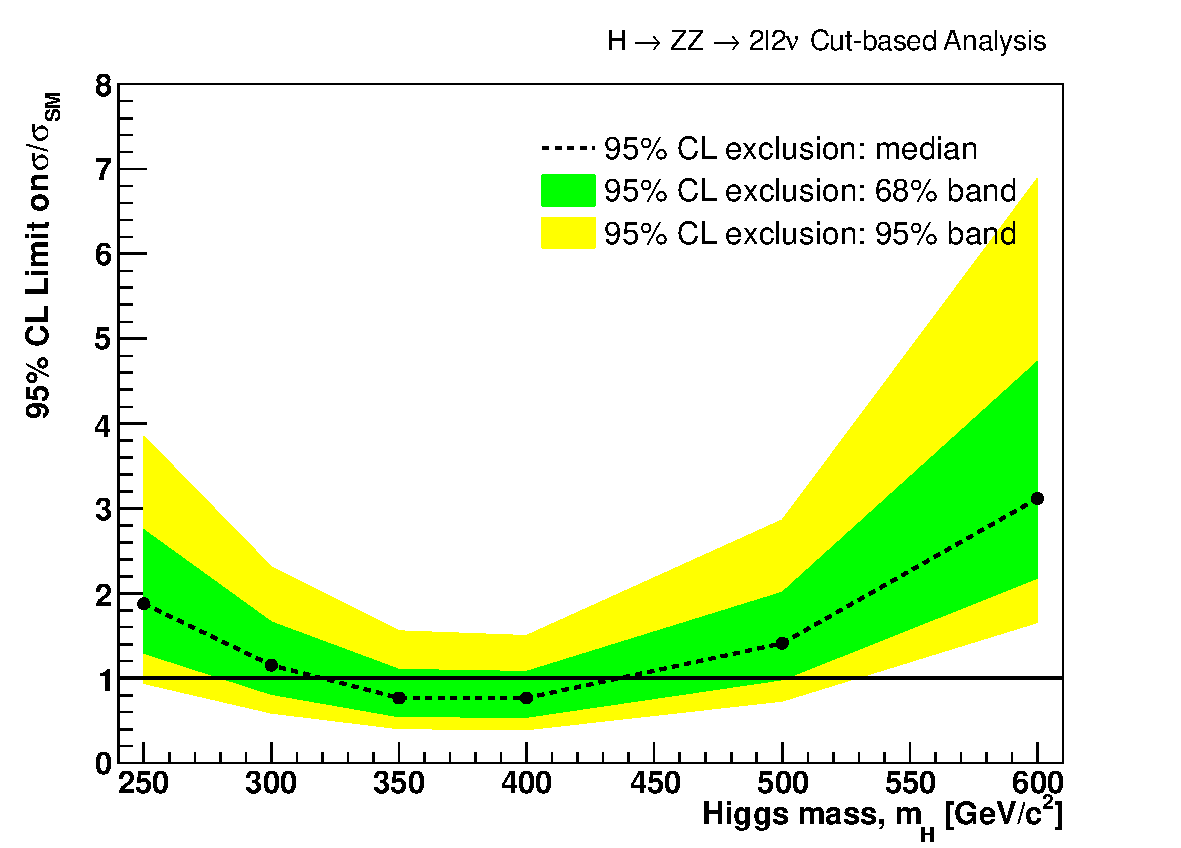
\includegraphics[width=0.6\textwidth]{figures/limits_cut_4fb.pdf}
   \caption{Cut-based analysis expected upper limits at 95\% C.L. for \intlumi\ of data. }
   \label{fig:limits_cut_4fb}
\end{center}
\end{figure}
%%%%%%%%%%%%%%%%%%%%%%%%%%%%%


\clearpage
